%%==============================================================
%% Autor: Matheus dos Reis de Jesus
%% Última versão Maio/2021
%% Arquivo em formato UTF-8
%% Compilar com pdftex
%% Precisa do arquivo abntex2-UFV.sty e abntex2cite.tex
%%
%% Modelo: Rodrigo Smarzaro (smarzaro@ufv.br)
%%==============================================================

\documentclass[
	% -- opções da classe memoir --
	12pt,				    % tamanho da fonte
	openright,			    % capítulos começam em pág ímpar (insere página vazia caso preciso)
	oneside,			    % para impressão só no anverso. Oposto a twoside
	a4paper,			    % tamanho do papel.
    % -- opções do pacote abntex2 --
    % chapter=TITLE,         % Títulos em maiúsculas
    sumario=tradicional,    % Sumário padrão memoir (mais bonito "imo")
    % -- opções do pacote babel --
	english,			    % idioma adicional para hifenização
	brazil,				    % o último idioma é o principal do documento
	]{abntex2}              % Personaliza a capa. Precisa do arquivo ufv.cls para funcionar.


		% Pacotes fundamentais
\usepackage{abntex2-UFV}        % Personalização para a Universidade Federal de Viçosa
\usepackage{lmodern}			% Usa a fonte Latin Modern			
\usepackage[T1]{fontenc}		% Selecao de codigos de fonte de saída
\usepackage[utf8]{inputenc}		% Codificacao do documento (conversão automática dos acentos)
\usepackage{indentfirst}		% Indenta o primeiro parágrafo de cada seção.
\usepackage{graphicx}			% Inclusão de gráficos
\usepackage{booktabs}           % \toprule, \midrule e \bottomrule para tabelas
% Sistema autor-data com títulos nas referências em negrito
\usepackage[alf,abnt-emphasize=bf]{abntex2cite}	

% ---
% CONFIGURAÇÕES DE PACOTES
% ---

% Informações de dados para CAPA e FOLHA DE ROSTO
\titulo{\emph{UI Framework em React Native acessível para idosos}}
\autor{Matheus dos Reis de Jesus}
\local{Viçosa}
\data{2020}
\orientador{Lucas Francisco da Matta Vegi}    % redefinido no abntex2-UFV para aceitar Instituição (default = UFV-CRP)
%\coorientador{Nome do Coorientador}
\instituicao{Universidade Federal de Viçosa}

\campus{\emph{Campus} de Viçosa}      % pacote abntex2-UFV
\curso{Ciência da Computação}               % pacote abntex2-UFV
%\membrobancaA{Membro da Banca A}             % pacote abntex2-UFV default = UFV-CRP
%\membrobancaB[UFMG]{Membro da Banca B}       % pacote abntex2-UFV default = UFV-CRP
%\databanca{\today}                           % pacote abntex2-UFV

% O preambulo deve conter o tipo do trabalho, o objetivo,
% o nome da instituição e a área de concentração
\preambulo{Projeto apresentado à Universidade Federal de Viçosa como parte das exigências para a aprovação na disciplina Seminários I}
% ---

% ---
% Configurações de aparência do PDF final

% informações para o arquivo pdf de saída
% Interessante alterar a cor dos links para preto(black)
% para imprimir
\makeatletter
\hypersetup{
        % metadados
		pdftitle={\@title},
		pdfauthor={\@author},
    	pdfsubject={\imprimirpreambulo},
	    pdfcreator={LaTeX with abnTeX2},
		colorlinks=true,   % false: links em frame; true: links coloridos
    	linkcolor=black,    % cor dos links no documento
    	citecolor=blue,    % cor dos links para a bibliografia
    	filecolor=magenta, % cor dos links para arquivos
		urlcolor=blue,     % cor dos links para sites
		bookmarksdepth=4   % profundidade do sumário do PDF
}
\makeatother
% ---

\begin{document}
% Retira espaço extra obsoleto entre as frases.
\frenchspacing

% ----------------------------------------------------------
% ELEMENTOS PRÉ-TEXTUAIS
% ----------------------------------------------------------
\pretextual

% Capa
\imprimircapa

% Folha de rosto
\imprimirfolhaderosto
% ---

% Inserir folha de aprovação
%\imprimirfolhadeaprovacao

% Dedicatória
%\begin{dedicatoria}
%   \vspace*{\fill}
%   \centering
%   \noindent
%   \textit{Texto qualquer da dedicatória}
%   \vspace*{\fill}
%\end{dedicatoria}
% ---

% Agradecimentos
%\begin{agradecimentos}

%\end{agradecimentos}
% ---

% Epígrafe
%\begin{epigrafe}
%    \vspace*{\fill}
%	\begin{flushright}
%		\textit{``Word? nunca mais.''\\
%		(Qualquer usuário de \LaTeX)}
%	\end{flushright}
%\end{epigrafe}
% ---

% RESUMOS

% resumo em português
%\begin{resumo}
% \noindent
%Insira o resumo aqui

%\vspace{\onelineskip}

%\noindent
% \textbf{Palavras-chaves}: React Native, Framework, UI , Acessibilidade, UFV.
%\end{resumo}

% resumo em inglês
%\begin{resumo}[Abstract]
% \begin{otherlanguage*}{english}
%   \noindent
%   % Insira o abstract aqui
%
%   \vspace{\onelineskip}
%
%   \noindent
%   \textbf{Key-words}: TCC, latex, abntex, UFV..
% \end{otherlanguage*}
%\end{resumo}

% inserir lista de ilustrações
%\pdfbookmark[0]{\listfigurename}{lof}
%\listoffigures*
%\cleardoublepage
% ---

% inserir lista de tabelas
%\pdfbookmark[0]{\listtablename}{lot}
%\listoftables*
%\cleardoublepage
% ---


% Lista de siglas e abreviaturas (opcional)
% sintaxe: \item [sigla] Descrição da sigla

%\begin{siglas}
%\item[ABNT] Absurdas Normas Técnicas
%\item[UFV] Universidade Federal de Viçosa
%\item[CRP] \emph{Campus} de Rio Paranaíba
%\end{siglas}

% Lista de símbolos (opcional)
% sintaxe: \item [simbolo] Descrição do símbolo

%\begin{simbolos}
%\item[$\infty$ ] Infinito
%\end{simbolos}


% inserir o sumario
\pdfbookmark[0]{\contentsname}{toc}
\tableofcontents*
\cleardoublepage
% ---

% ----------------------------------------------------------
% ELEMENTOS TEXTUAIS
% ----------------------------------------------------------
\textual


%Modifique a estrutura dos capítulos e seções de acordo com a necessidade do seu trabalho
\chapter{Apresentação}\label{sec:apresentacao}

		Este projeto foi idealizado ao observar, repetidas vezes, meu avô apresentar dificuldades para executar determinadas ações usando um dispositivo móvel. Ao me deparar com isso, lembrei que pessoas da terceira idade geralmente apresentam dificuldade em redigir e ler textos, interagir com campos de entrada ou imagens, seja utilizando um dispositivo mais simples ou um \textit{smartphone}.

\par

Além do fator idade, existem diversas doenças que tornam ainda mais difíceis as interações de uma pessoa idosa com um dispositivo móvel. Problemas motores, de visão e cognitivos influenciam na capacidade de executar ações que são essencias para possibilitar o uso de tais dispositivos. Dito isso, surge uma necessidade de propor soluções que sejam capazes de sanar essas dificuldades.

		\par

\chapter{Referencial Teórico}\label{sec:referencialTeorico}		

		Em uma conversa com o orientador deste projeto, Lucas Vegi, conheci a tese de mestrado desenvolvida pela Dâmaris Arruda: Um \textit{framework} para facilitar as interações entre dispositivos móveis e pessoas idosas.

\par

		Em seu trabalho, Dâmaris buscou elencar as ações em dispositivos móveis que os idosos enfrentam maior dificuldade para executar. Após testes realizados em um trabalho conjunto com o \emph{Programa da Terceira Idade}, um projeto da Prefeitura Municipal de Viçosa - MG, foram identificadas tais ações: movimento de pinça, movimento de rotação e digitação.

Dadas as informações obtidas pelos testes realizados, foi então desenvolvido um \textit{framework} de interface de usuário nativo para \textit{Android}. O projeto contém um conjunto de componentes visuais com o objetivo de facilitar ações que geralmente exigem mais coordenação motora e acuidade visual.

\par

\chapter{Justificativa}\label{sec:justificativa}

Com o crescimento vertiginoso do uso de dispositivos móveis, há um aumento da demanda por aplicações que possam atender às mais diversas necessidades das pessoas que os utilizam. Segundo a \emph{31ª Pesquisa Anual de Uso de TI}, realizada pela \emph{Fundação Getúlio Vargas}, que pode ser consultada na seção de referências deste documento, publicada em junho de 2020, o Brasil já conta com pelo menos 342 milhões de dispositivos móveis, equivalente a 1,6 dispositivo móvel por habitante.

\par

	Como citado anteriormente, em sua Tese, Dâmaris criou um \textit{framework} de interface de usuário nativo para \textit{Android}, e isso limita a utilização do artefato produzido. A escolha do tema deste projeto foi feita buscando possibilitar o uso da ferramenta em diferentes plataformas.

\par

\chapter{Objetivo}\label{sec:objetivo}

Dado o fato de que o \textit{framework} criado pela Dâmaris tem uso limitado apenas em aplicações nativas da plataforma \textit{Android}, a proposta deste trabalho é implementar a mesma ferramenta usando uma tecnologia de desenvolvimento híbrido, que possibilite a utilização em múltiplas plataformas, como \textit{Android} e \textit{iOS}, sem necessidade de escrever implementações específicas para cada uma delas.

\chapter{Metodologia}\label{sec:metodologia}		

Através de pesquisas em diferentes fontes e uma análise minusciosa, a tecnologia híbrida escolhida para desenvolvimento deste \textit{framework} foi \textit{React Native}, que atualmente é mantido pelo \textit{Facebook}, e é utilizado em aplicações amplamento utilizadas, como \textit{Instagram}, \textit{AirBnb} e \textit{Uber}. A imagem a seguir mostra que o repositório do \textit{React Native}, no \textit{GitHub}, tem a maior quantidade de \textit{forks} e o segundo maior número de \textit{stars} e \textit{issues}, quando comparado com outras tecnologias de desenvolvimento híbrido, a saber: \textit{Flutter},\textit{Ionic} e \textit{Kivy}.

	\par

\begin{figure}[h]
	\begin{center}	
		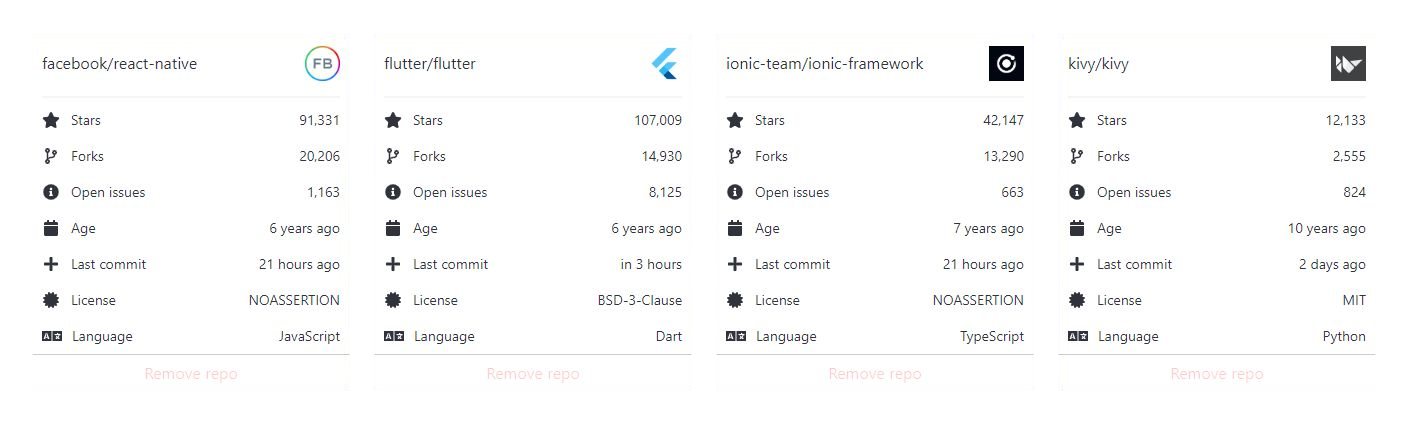
\includegraphics[width=.9\linewidth]{github-compare.png}
	\end{center}
	\caption[GitHub Compare]{Comparação entre as estatísticas dos repositórios de tecnologias de desenvolvimento híbrido: \textit{React Native}, \textit{Flutter}, \textit{Ionic} e \textit{Kivy}}
	\label{fig:githubCompare}
	\legend{Fonte: \textit{GitHub Compare}. Disponível em https://githubcompare.com/}
\end{figure}

\par
		
No \textit{ElderlyFrame}, nome dado ao projeto citado anteriormente neste trabalho, foram implementados componentes que facilitam atividades de zoom, rotação de elementos e também digitação de texto. A proposta do \emph{react-native-elderly}, nome dado ao artefato que será produzido ao fim deste trabalho, é implementar o mesmo conjunto de componentes utilizando a biblioteca \textit{React Native}.		 

\chapter{Cronograma}\label{sec:cronograma}

Para execução deste projeto, estão estipuladas abaixo as tarefas e os momentos em que elas serão realizadas, assim como o total de horas para cada grupo de atividades. Na tabela a seguir temos o planejamento para os 8 meses pelos quais este trabalho irá se estender:

\par

\begin{table}[htbp]
  \centering
    \caption[Cronograma mensal]{Cronograma do Projeto em Meses}
    \label{tab:cronogramaMensal}
    \begin{tabular}{lcccccccc} %|c|c|c|c|c|c|c|c|c|c|c|c
    \toprule
    \textbf{Atividade} & \textbf{1} & \textbf{2} & \textbf{3} & \textbf{4} & \textbf{5} & \textbf{6} & \textbf{7} & \textbf{8} \\
    \midrule
        Análise do Tema & $\bullet$ & $\bullet$ & & & & & &\\
        Revisão Literária & & $\bullet$ & $\bullet$ & & & $\bullet$ & $\bullet$ & $\bullet$ \\
        Projeto & & & $\bullet$ & $\bullet$ & $\bullet$ & $\bullet$ & $\bullet$ & $\bullet$ \\
        Desenvolvimento & & & $\bullet$ & $\bullet$ & $\bullet$ & $\bullet$ & & \\
        Documentação & & & $\bullet$ & $\bullet$ & $\bullet$ & $\bullet$ & & \\
    \bottomrule
    \end{tabular}
    \fonte{Próprio Autor}
\end{table}

As demandas de tempo(em horas) estimadas para orientação, desenvolvimento e revisão da literatura, do projeto escrito e demais artefafos produzidos são:

\par

\begin{table}[htpb]
	\centering
	\caption[Cronograma em horas]{Estimativa de tempo para cada atividade}
	\label{tab:cronogramaHoras}
	\begin{tabular}{lcc}
	\toprule
		\textbf{Item} & \textbf{Custeio} & \textbf{Tempo(horas)} \\
	\midrule
		Orientação & Governo Federal & 40 \\
		Projeto & Próprio & 60 \\
		Revisão & Próprio & 20 \\
	\bottomrule
		Total & & 120
	\end{tabular}
	\fonte{Próprio autor}
\end{table}

\chapter{Orçamento}\label{sec:orcamento}

Estão orçados para este projeto os itens contidos na tabela abaixo, acompanhados de  seus respectivos financiadores e valores:

\par

\begin{table}[htpb]
	\centering
		\caption[Orçamento]{Orçamento financeiro}
		\label{tab:orcamento}
		\begin{tabular}{lccc}
		\toprule
		\textbf{Item} & \textbf{Custeio} & \textbf{Custo} \\
		\midrule
			Computador Pessoal & Próprio & R\$ 5000  \\
			Conexão com a \textit{Internet} & Próprio & R\$ 900 \\
			Licença para publicação na Play Store & Próprio & ~R\$140 \\
		\bottomrule
			Total & & R\$6040 \\
		\end{tabular}%
		\fonte{Próprio Autor}
\end{table}%

% \chapter{Resultados Esperados}\label{sec:resultEsperados}

% ----------------------------------------------------------
% ELEMENTOS PÓS-TEXTUAIS
% ----------------------------------------------------------
        \postextual

% Referências bibliográficas
\bibliographystyle{abbrv}
\bibliography{referencias}
		
% Caso sejam necessários apêndices ou anexos em seu documento
% Use os ambientes abaixo

%% Apêndices
%
%% Inicia os apêndices
%\begin{apendicesenv}
%
%% Imprime uma página indicando o início dos apêndices
%\partapendices
%
%\chapter{Primeiro Apêndice}
%
%\chapter{Segundo Apêndice}
%
%\end{apendicesenv}
%
%
%% ----------------------------------------------------------
%% Anexos
%% ----------------------------------------------------------
%\begin{anexosenv}
%
%% Imprime uma página indicando o início dos anexos
%\partanexos
%
%\chapter{Primeiro Anexo}
%\lipsum[30]
%
%\chapter{Segundo Anexo}
%\lipsum[31]
%
%\end{anexosenv}

\end{document}